%!TEX TS-program = xelatex
%!TEX encoding = UTF-8 Unicode
\documentclass[11pt,a4paper]{article}

%\usepackage[left=70pt,top=50pt,bottom=70pt,right=40pt]{geometry}
\usepackage{amsmath}
\usepackage{amsfonts}
\usepackage{amssymb}
\usepackage{fixltx2e}
\usepackage{cmap}
\usepackage{enumerate}
\usepackage{ifthen}
\usepackage{listings}
\usepackage{url}
\usepackage[T1]{fontenc}
%\usepackage{fontspec}
%\usepackage{xunicode}
%\usepackage{xltxtra}
%\setmainfont[Mapping=tex-text,Ligatures={Common,Rare,Discretionary}]{Linux Libertine O}
\usepackage{pdflscape}
\usepackage{alltt}
\usepackage{algpseudocode}
\usepackage{subfigure}
\usepackage{graphicx}
\usepackage{verbatim}

\ifthenelse{\isundefined{\hypersetup}}{
    \usepackage[colorlinks=true,linkcolor=blue,urlcolor=blue]{hyperref}
    \urlstyle{same}
}{}

\hypersetup{
    pdftitle={Intelligent Agents - EX3 - Yoan Blanc, Tiziano Signo}
}
\title{\phantomsection%
    A Centralized Agent for the Pickup and Delivery Problem
}
\author{
    \textbf{Group 16}\\
    Yoan Blanc \texttt{<yoan.blanc@epfl.ch>}, 213552\\
    Tiziano Signo \texttt{<tiziano.signo@epfl.ch>}, 226511
}
\date{\today}


\begin{document}
\maketitle

\noindent
\begin{quote}{\it

    In this exercise you will implement the Stochastic Local Search algorithm
    (SLS) to find an efficient solution to the CSP description of the PDP.

    \begin{enumerate}
        \item Implement the Stochastic Local Search algorithm for the PDP.

        \item Run simulations for different configurations of the environment
        (i.e. different tasks and number of vehicles) in order to observe the
        behavior of the centralized planner using the SLS algorithm.

        \item Reflect on the fairness of the optimal plans. Observe that
        optimality requires some vehicles to do more work than others.
        Illustrate this observation with an example in your report.

        \item Test your program for different number of vehicles and various
        sizes of the task set. How does the complexity of your algorithm depend
        on these numbers?

    \end{enumerate}

}\end{quote}

\newpage
\subsection*{Implementation}

The system is composed of $N_T$ tasks that has to be picked up from a city
and delivered to another city. There is $N_V$ vehicles that are carrying a
plan to handle a subset of the tasks.

\subsubsection*{State representation}

Every task $t_i$ is split into two actions: $p$ (pickup) and $d$ (delivery).

\begin{align*}
actions = \{&t_1^p,                               & \text{task $1$ pickup} \\
            &t_1^d,                               & \text{task $1$ delivery} \\
            &t_2^p, &_2^d,                        & \\
            &\dots,                               & \\
            &t_{N_T}^p, t_{N_T}^d\}               & \text{up to the end}
\end{align*}

The set of plans is formed of tuples, one per vehicle, and the corresponding
list of action to do. This is as strong constraints that:

\begin{enumerate}
    \item two actions from a same task must be in the same plan,

    \item pickup and delivery must appear in that order,

    \item each item appear once and only once among the plans.
\end{enumerate}

\begin{align*}
plans = \{&(v_1, (t_j^p, t_j^d, \: \dots)),            & \text{vehicle $1$ and task $j$} \\
          &(v_2, (t_k^p, t_l^p, \dots, t_k^d, t_l^d)), & \text{interleaved tasks} \\
          &\dots,                                      & \\
          &(v_{N_V}, \varnothing)\}                    & \text{actions can be empty too}
\end{align*}

\subsubsection*{Algorithm}

The algorithm is quite straightforward. Thus we would like to explain in more
depth the \textsc{chooseNeighbors} function. Instead of doing two things:
moving one task from one schedule to another one and reorder one schedule, it's
computing all the possible positions across all schedules for a task. To do so,
the task is removed from the plan and the inserted at the acceptable positions
(without taking care of the vehicle's capacity). If a schedule has $t$ tasks,
there is $(2t - 1)t$ different positions. The overall cost is $O(|S| \cdot
(\frac{|T|}{|S|})^2) \approx O(|T|^2)$ which was expected.

We've played with two strategies for the \textsc{initialSolution} part:

\begin{enumerate}
    \item \textbf{All tasks to the biggest agent}\\
        This solution seems to converge quickly and give better solution
        overall. The downside is that it has no incentives to split the tasks
        among other vehicles. (See \emph{Fairness} below)

    \item \textbf{Round-robin assignement of tasks}\\
        This solution usually gives worse result than the previous all-to-one
        idea but enlighten why better solutions require less agent. Hence, we
        didn't keep it as the default way of populating the initial plan.

\end{enumerate}

\begin{comment} % Takes too much space
\begin{algorithmic}
    \Function{SLS}{$vehicles, tasks$}
        \State $plan \gets $ \Call{initialSolution}{$vehicles, tasks$}
        \While{$not finished$} % FIXME
            \State $neighbors \gets $ \Call{chooseNeighbors}{$plan$}
            \State $plan \gets $ \Call{localChoice}{$plan, neighbors$}
        \EndWhile
        \State \Return $plan$
    \EndFunction


    \Function{initialSolution}{$vehicles, tasks$}
        \State $plan \gets \varnothing$
        \ForAll{$vehicle \: \in \: vehicles$}
            \State $plan = plan \cup (vehicle, \varnothing)$
        \EndFor
        \ForAll{$task \: \in \: tasks$}
            \State Assign the task to a vehicle's schedule in a round-robin fashion.
        \EndFor
    \EndFunction

    \Function{chooseNeighbors}{$plan$}
        \State $neighbors \gets \varnothing$
        \State $task \gets $ \Call{pickRandomTask}{$plan$}
        \ForAll{$schedule \: \in \: plan$}
            \ForAll{$(p, d) \: \in $ \Call{taskPosition}{$schedule$}}
                \State $neighbor \gets $ \Call{clone}{$plan$}
                \State \Call{removeTaskFromPlan}{$neighbor, task$}
                \State \Call{addTaskToPlan}{$neighbor, task, (p, d)$}
                \State $neighbors \gets neighbors \cup neighbor$
            \EndFor
        \EndFor
        \State \Return $neighbors$
    \EndFunction

    \Function{localChoice}{$plan, neighbors$}
        \State $best \gets plan$
        \ForAll{$neighbor \: \in \: neighbors$}
            \If{\Call{isValid}{$neighbor$} $\wedge$ \Call{cost}{$best$} $\ge$ \Call{cost}{$neighbor$}}
                \State $best \gets neighbor$
            \EndIf
        \EndFor
        \State \Return $best$
    \EndFunction
\end{algorithmic}
\end{comment}

\subsection*{Behaviour}

Since there is no time constraints here, the algorithm tends to assign all the
tasks to one agent. It can be very simply explained by the fact that as soon as
one agent reaches another agent's starting point. It become as good as the
later (assuming its maximal capacity is not reached yet).


\subsection*{Optimality \& Fairness}

Optimality means travelling a very few to deliver a maximum stuff. A way to
look at it is the display the load over time (or travelling distance). We see
in Figures~\ref{fig:one1} and \ref{fig:rr1} that the final plans try to be on
high load as much as possible.

\begin{figure}[ht!]
    \begin{center}
    \subfigure[Initial state]{
        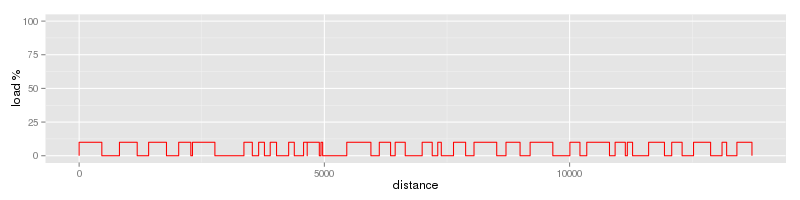
\includegraphics[width=1\textwidth]{plan_2662_0.png}
        \label{fig:one0}
    }
    \subfigure[Final state]{
        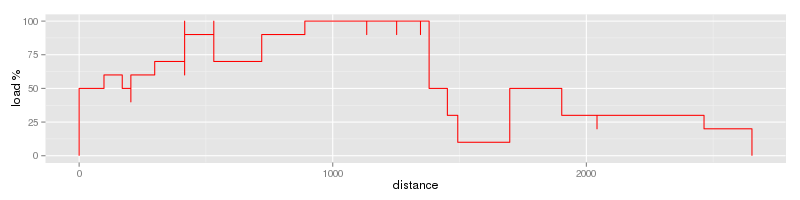
\includegraphics[width=1\textwidth]{plan_2662_1.png}
        \label{fig:one1}
    }
    \caption{All the tasks go to one agent}{Total distance travelled: $2662$}
    \label{fig:one}
    \end{center}
\end{figure}


\begin{figure}[ht!]
    \begin{center}
    \subfigure[Initial state]{
        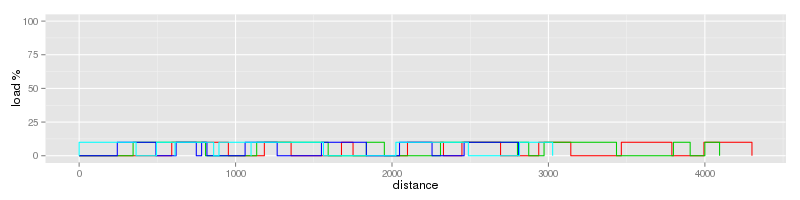
\includegraphics[width=1\textwidth]{plan_2861_0.png}
        \label{fig:rr0}
    }
    \subfigure[Final state]{
        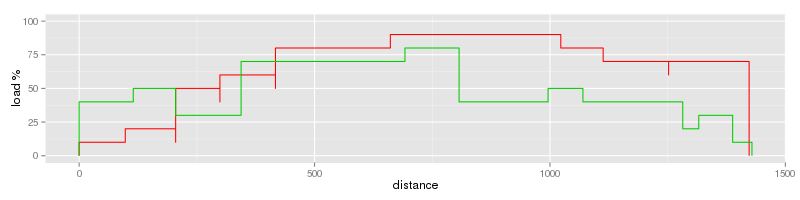
\includegraphics[width=1\textwidth]{plan_2861_1.png}
        \label{fig:rr1}
    }
    \caption{Round-robin distribution of the tasks}{Total distance travelled: $2861$}
    \label{fig:rr}
    \end{center}
\end{figure}

Regarding the fairness, if the algorithm tends to reduce the number of vehicles.
Even with the round robin initial setup (see Figure~\ref{fig:rr}), the output solution
kept only two vehicles and none of them managed to get fully loaded.

One explanation is that for every vehicle there is a \emph{loading up} phase
where it's collecting tasks to be delivered (maximizing the reward per km) at
the beginning and an \emph{unloading} one at the end. Only the core of the
vehicle's plan (where its load is high, let's say $>50\%$) tends to an optimal
solution while both the beginning and the end cannot be.

\subsection*{Algorithm complexity}

As explained before, the complexity is of $O(|T|^2)$ for each step and does not
depend on the number of vehicles.

\textbf{to be continued\ldots}

\end{document}
